\documentclass{article}
\usepackage{amsfonts, amsthm, amsmath}

\usepackage{geometry, graphicx}
\usepackage{algorithm, algorithmic}
\usepackage{bm}
\usepackage{multirow}
\geometry{left = 5em, right = 5em}

\def\showtopic{Mathematical Image Processing Homework 1}
\def\showtitle{Variational Methods for Image Restoration}
\def\showabs{Total Variational Model}
\def\showauthor{Yuanfeng Shi, 1800010697}

\title{\showtitle}
\author{\showauthor}

\usepackage{fancyhdr}  
\pagestyle{fancy}
\lhead{\textbf {\showtopic} }
\chead{} 
\rhead{\textbf {\showabs} }
\lfoot{} 
\cfoot{\thepage}
\rfoot{} 
\renewcommand{\headrulewidth}{0.4pt} 


\usepackage{listings}
\lstset{language=Matlab}
\lstset{breaklines}
\lstset{extendedchars=false}
\newtheorem{proposition}{Proposition}
\newtheorem{remark}{Remark}
\begin{document}
\maketitle
\thispagestyle{fancy}

\section{Finite Difference Approximation of Derivatives}

Difference among different discretizations (h=1)
\begin{equation}\nonumber
\Delta v|_{i,j}\simeq \lambda \frac{v_{i+1,j}+v_{i-1,j}+v_{i,j+1}+v_{i,j-1}-4v_{i,j}}{h^2}+(1-\lambda) \frac{v_{i+1,j+1}+v_{i-1,j+1}+v_{i+1,j-1}+v_{i-1,j-1}-4v_{i,j}}{2h^2}
\end{equation}
The second approximation of derivatives can be seen as the 45 degree rotation of the first approximation, and its step size is $\sqrt{2} h$. Consider
\begin{equation}\nonumber
(1-\lambda)\frac{v_{i+1,j+1}+v_{i-1,j+1}+v_{i+1,j-1}+v_{i-1,j-1}-4v_{i,j}}{{(\sqrt{2} h)}^2}
\end{equation}
In order to make the norms of different discrete gradients are equal, $2*(1-\lambda)=\lambda, \lambda = \frac{2}{3}$.
 
As for the first order,
\begin{equation}\nonumber
\frac{\partial v}{\partial x}|_{i,j}\simeq \lambda \frac{v_{i+1,j}-v_{i-1,j}}{2h}+\frac{(1-\lambda)}{2} (\frac{v_{i+1,j+1}-v_{i-1,j+1}}{2h}+\frac{v_{i+1,j-1}-v_{i-1,j-1}}{2h})
\end{equation}
$\sqrt{2}*(1-\lambda)=\lambda, \lambda = 2-\sqrt{2}$.

\section{Introduction}

Image restoration, including image denoising, deblurring, superresolution,
\emph{etc.}, is one of the most important areas in imaging science.
Its major purpose is to obtain high quality reconstructions of images
corrupted in various ways during imaging, acquisiting and storing.
The basic linear restoration model is usually characterized as solving the inverse problem
\begin{equation}
f = Au+\eta
\end{equation}

The  fundamental problem in image reconstruction is to design an appropriate regularization to characterize natural images. Rudin and Osher introduced a regularization term, and the functional is like:
\begin{equation}
E_{ROF}(u) := \|f-Au\|_{L^2(\Omega)} + |u|_{TV(\Omega)}. 
\end{equation}
Here the Total Variation (TV) seminorm is a generalization of the integration of the derivative of $u$: $\int_{\Omega}|u'|$. The ROF model can preserve the edge while deblur or denoise in the subdomain successfully. 

To solve the ROF method, we use the Split Bergman method.

\section{Split Bregman Method}
The Split Bregman method is a technique for solving a variety of L1-regularized optimization problems, and is particularly effective for problems involving total-variation regularization.  Split Bregman is one of the fastest solvers for Total-Variation denoising, image reconstruction from Fourier coefficients, convex image segmentation, and many other problems.  The method is a re-interpretation of the alternating direction method of multipliers that is specially adapted to L1 problems.   

Let us consider a general case:

\begin{equation}
\min \|\lambda \cdot Wu\|_1 + H(u),
\end{equation}
where $W$ is a $n\times n$ matrix and $H$ is convex and differentiable. We begin with a simple substitution:
$$\min_{u,d} \|\lambda \cdot d\|_1 + H(u)\quad s.t. \quad d = Wu.$$
Recall the Augmented Lagrangian:
$$\mathcal{L}_{\mu}(u,d,p) = \|\lambda \cdot d\|_1 + H(u) + p^T(d-Mu) + \frac{\mu}{2}\|Wu-d\|_2^2.$$

Solving the saddle point problem by:
$$\left\{
\begin{array}{rl}
(u_{k+1},d_{k+1}) &= argmin_{u,d}\|\lambda \cdot d\|_1 + H(u) + p_k^T(d-Mu) + \frac{\mu}{2}\|Wu-d\|_2^2\\
p_{k+1} &= p_k + \delta\mu(d_{k+1} - Wu_{k+1})
\end{array}
\right.
$$
Which is equivalent to the following subroutine:
$$\left\{
\begin{array}{rl}
(u_{k+1},d_{k+1}) &= argmin_{u,d}\|\lambda \cdot d\|_1 + H(u) +  \frac{\mu}{2}\|Mu-d+b_k\|_2^2\\
b_{k+1} &= b_k + \delta(Wu_{k+1} - d_{k+1})
\end{array}
\right.
$$

\section{Detailed Algorithm}

We use the discretization in Section 1. Assume $u$ is a function defined on $[0,1]^2$.

Define the space with grid size $h:=\frac 1n$:
\begin{equation}
\Omega_n := \{(\frac in,\frac jn)\in [0,1]^2:i,j\in \mathbb Z\}
\end{equation}
equipped with the following norm :
\begin{equation}
\|\bm{v}\|_{p,n} := \big(\sum_{i=0,j=0}^{n}|\bm{v}(i,j)|^p\big)^{1/p}
\end{equation}
Then the discrete functional is proposed as:
\begin{equation}
E_n(\bm{u}) = \frac 12\|\bm{A}\bm{u}-\bm{f}\|_{2,n}^2 + \frac{\lambda}{2}\big[\|\frac{\partial}{\partial x}\bm{u}\|_{1,n} + \|\frac{\partial}{\partial y}\bm{u}\|_{1,n} \big].
\end{equation}
And it can be approximately realized by a $2n \times n$ matrix $W$:
\begin{equation}
\label{En}
E_n(\bm{u}) = \frac 12\|\bm{A}\bm{u}-\bm{f}\|_{2,n}^2 + \frac{\lambda}{2}\|\bm{W}\bm{u}\|_{1,n} .
\end{equation}
To solve \eqref{En}, we adopt the Split Bregman Algorithm introduced in Section 3. For simplicity, we drop the subscript $n$ when the grid size is fixed More explicitly, let $H(\bm{u}) = \frac 12\|\bm{A}\bm{u}-\bm{f}\|_2^2,$ we get
$$
\left\{\begin{array}{rl}
\bm{u}_{k+1} &= argmin_{\bm{u}} \frac 12\|\bm{A}\bm{u}-\bm{f}\|_2^2 +\frac{\mu}{2} \|\bm{W}\bm{u} - \bm{d}_{k} + \bm{b}_{k}\|_2^2 \\ 
\bm{d}_{k+1} &=argmin_{\bm{d}}\lambda \|\bm{d}\|_1 + \frac{\mu}{2} \|\bm{d} - \bm{W}\bm{u}_{k+1} - \bm{b}_{k}\|_2^2 \\
\bm{b}_{k+1} &= \bm{b}_{k} + \delta (\bm{W}\bm{u}_{k+1} - \bm{d}_{k+1})
\end{array}
\right.
$$

Each step in the subroutine has an explicit solution, so we obtain the efficient algorithm:
\begin{algorithm}
\caption{Split Bregman For Analysis Approach}
\begin{algorithmic}[1]
\STATE set $\bm{d}_0$, $\bm{b}_0$ as zero.
\STATE $\bm{u} = \bm{f}$ 
\REPEAT
\STATE $\bm{u}_{k+1} = \big[\bm{A}^T\bm{A} + \mu \bm{W}^T\bm{W} \big]^{-1}[\bm{A}^T\bm{f} + \mu \bm{W}^T(\bm{d}_{k} - \bm{b}_{k})]$
\STATE $\bm{d}_{k+1} = \mathcal{T}_{\lambda/\mu}(\bm{W}\bm{u}_{k+1} + \bm{b}_{k})$
\STATE $\bm{b}_{k+1} = \bm{b}_{k} + \delta(\bm{W}\bm{u}_{k+1} - \bm{d}_{k+1})$
\UNTIL{$\frac{\|\bm{W}\bm{u}_{k+1}-\bm{d}_{k+1}\|}{\|f\|_2} < tol$ or achieve maximal iter}
\end{algorithmic}
\end{algorithm}

\begin{remark}
\begin{enumerate}
\item $\mathcal{T}_{\alpha}$ is the soft thresholding function $x \mapsto \frac{x}{|x|}\max(x-\alpha,0)$
\item In general, we use the sparse matrix to lower the computitional complexity.
\item We use the function gmres for sparse matrix to solve the calculation of $\bm{u}$.
\item The more details of the algorithm is shown in the MATLAB code.
\end{enumerate}
\end{remark}

\section{Numerical Result}
In this section, we conduct some numerical simulations on image deblurring.We test the algorithm in different blur settings and noise settings. The convolution operator is generated by “fspecial” function in MATLAB and the noise is generated by “randn” function. For the quantitative comparison, we calculate the peak signal to noise ratio (PSNR) value and the SSIM value, and the results are below. 
         
        \begin{center}
                   \begin{tabular}{|c|c|c|c|c|c|c|c|}
                      \hline
                       noise & index & \multicolumn{3}{|c|}{peppers256} & \multicolumn{3}{|c|}{barbara}\\
                      \hline
                         & & Origin & End & Max & Origin & End & Max \\
                      \hline
                       \multirow{2}{*}{0.01} 
                         & PSNR & 24.79 & 29.80 & 30.02 & 24.98 & 28.17 & 28.24 \\
                         & SSIM & 0.8641& 0.8895& 0.8911& 0.7559& 0.8221& 0.8431 \\
                      \hline
                       \multirow{2}{*}{0.01} 
                         & PSNR & 24.53 & 27.97 & 28.12 & 24.51 & 26.54 & 26.68 \\
                         & SSIM & 0.7566& 0.7977& 0.8031& 0.6752& 0.7304& 0.7607 \\ 
                      \hline
                   \end{tabular}
        \end{center}

\begin{figure}[H]
\centering
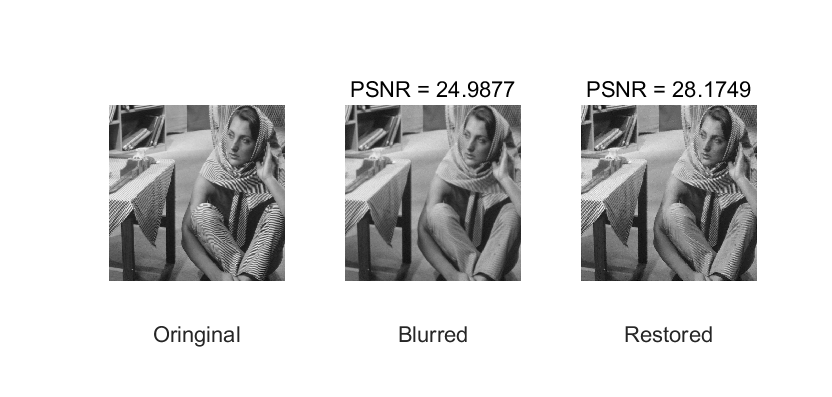
\includegraphics[scale=0.8]{1.png}
\caption{Image 'barbara': kernel = fspecial(15,1) noise = 0.01*randn(n*n)}
\centering
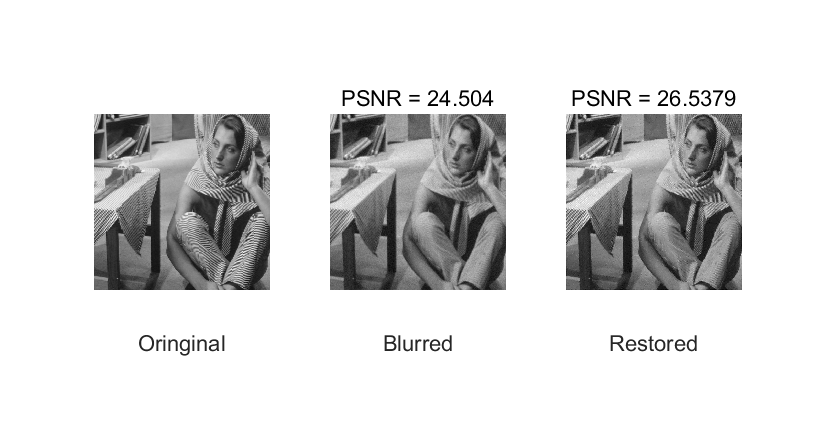
\includegraphics[scale=0.8]{2.png}
\caption{Image 'barbara': kernel = fspecial(15,1) noise = 0.02*randn(n*n)}
\end{figure}

\begin{figure}[H]
\centering
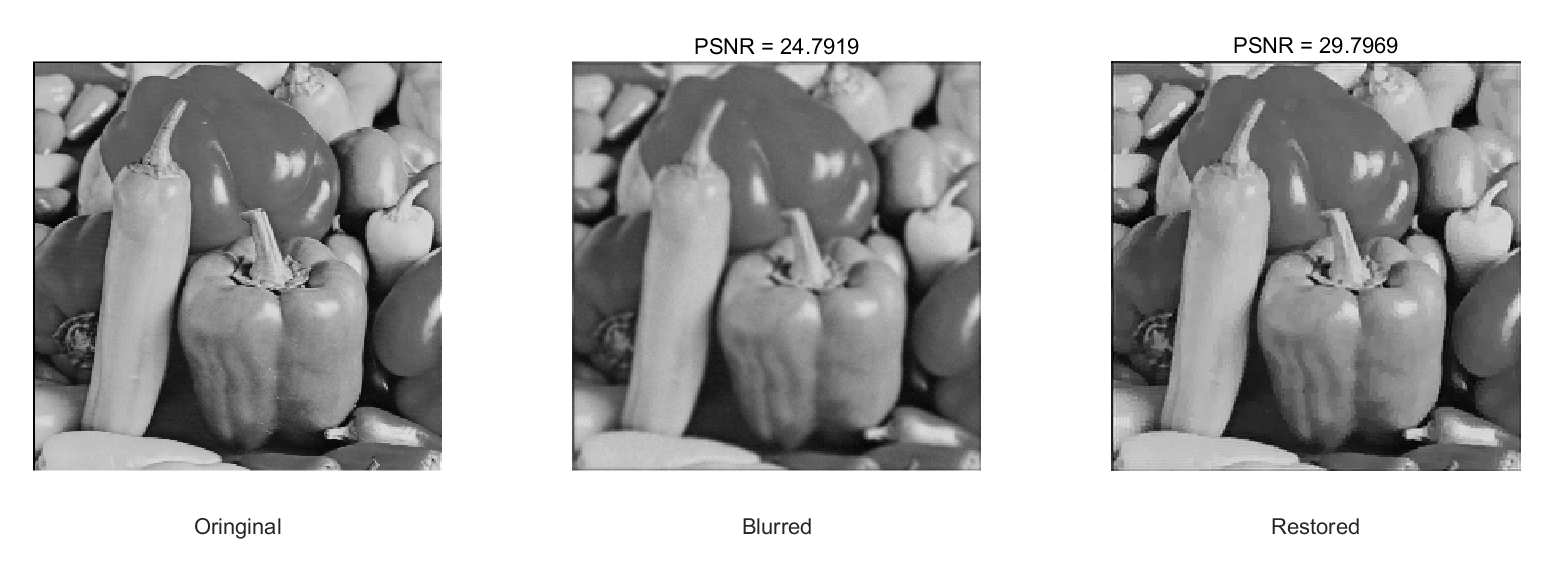
\includegraphics[scale=0.4]{3.png}
\caption{Image 'peppers256': kernel = fspecial(15,1) noise = 0.01*randn(n*n)}
\centering
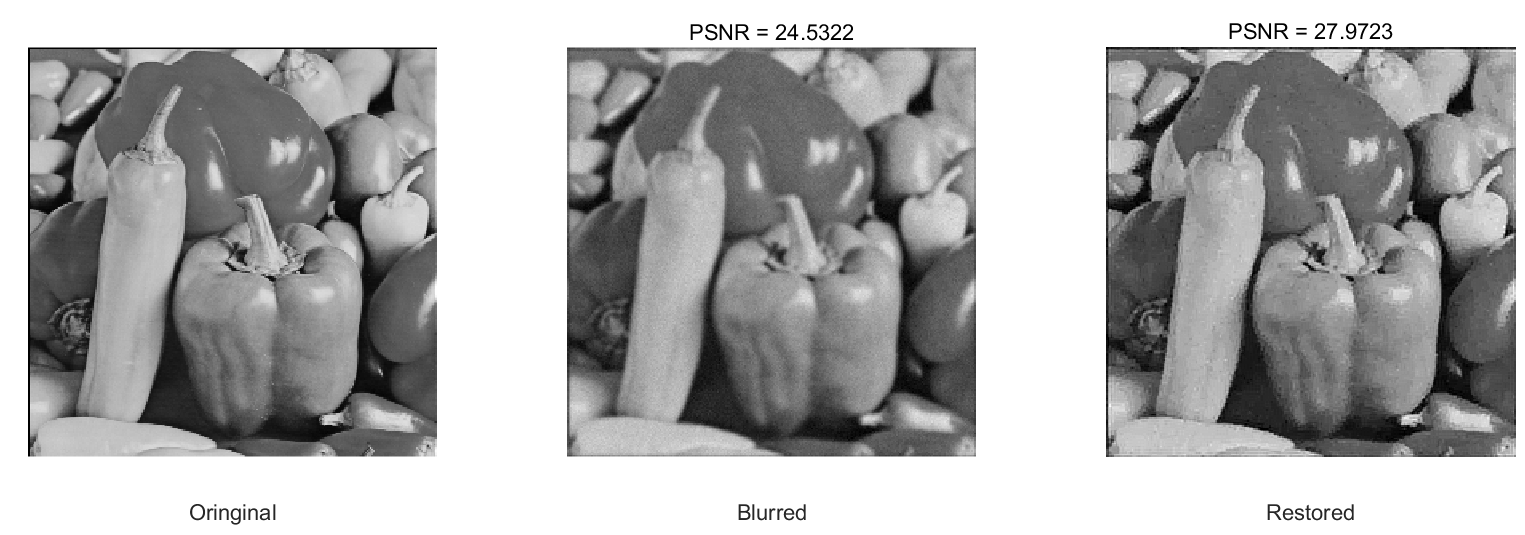
\includegraphics[scale=0.4]{4.png}
\caption{Image 'peppers256': kernel = fspecial(15,1) noise = 0.02*randn(n*n)}
\end{figure}

\end{document}